\documentclass{article}
\usepackage[T1]{fontenc}
\usepackage[utf8]{inputenc}

\usepackage{amsmath,amssymb,graphicx}
\usepackage{tikz}
\usetikzlibrary{automata,positioning,arrows,arrows.meta} % arrows.meta gives “stealth'”

\title{EECS 510 Final Project: Zelda Character Interactions}
\author{Ian Collins \and Abdelrahman Zeidan \and Del Endecott}
\date{April 2025}

\DeclareUnicodeCharacter{202F}{\,}

\begin{document}
\maketitle
\centering{https://github.com/Ian-Collins1252/EECS510Final}
%--------------------------------------------------------------------
\pagebreak
\subsection{Project Description}

\quad Our project aimed to describe the different interactions that are possible within the Legend of Zelda series of video games made by Nintendo. The interactions we modeled were between Link, the main protagonist, some NPCs (nonplayable characters) like Impa and Zelda, and some battles Link encounters like Ganondorf. We decided to model each of these interactions within a Python script, utilizing class structure to manage who is in the interaction, as well as manage that given characters vocabulary. Each of these interactions are modeled below using NFAs and a Turing machine. NFAs describe the different states and transitions for each of the characters. NFAs additionally describe the dialog chain that Link has with different NPCs. NPC dialog usually offers some exposition about the world while offering Link the opportunity to accept a quest from that character. Link can request more information, accept the quest, and decline the quest. Link does have a unique interaction with Zelda, where she can feed Link, and following this, Link will open up about his backstory. This references both Link's love for food in the Breath of the Wild line of games as well as Zelda's diary in Breath of the Wild found in her bedroom. This diary has an entry describing how Zelda got Link to open up about his past and why he remains silent despite being one of the most important people in Hyrule.\\
\quad Link's battle system is modeled with a Turing machine utilizing 4 separate tapes to track Link's health, opponent's health, Link's actions, and the opponent's actions. Link will win or retreat in these interactions based on the remaining amount of health and actions he can take. These actions Link can take vary from attack, spin attack, shield, and bomb which all have unique interactions with the opponent character. Win cases are either the opponent losing all of their health or having no more actions to perform. Lose conditions are the same if Link loses all of his hearts or runs out of actions. The Turing machine is constructed using tape objects nested within the machine. The tape can navigate left or right while reading and writing the current character. The machine models the different actions which can occur within the battle simulation. We can determine the state of the end of the battle after the simulation.
%--------------------------------------------------------------------
\subsection*{Dialogue vocabularies}

\[
\begin{aligned}

\text{Link}\; &= \{\texttt{idle},\texttt{hi},\texttt{yes},\texttt{no},\texttt{tell},\texttt{fight},\texttt{win},\texttt{retreat},\texttt{eat},\texttt{backstory},\texttt{bye}\}\\[4pt]

\text{Zelda}\; &= \{\texttt{idle},\texttt{hi},\texttt{Exp},\texttt{Quest},\texttt{Feed},\texttt{bye}\}\\[4pt]

\text{Ganon}\; &= \{\texttt{idle},\texttt{lie},\texttt{win},\texttt{lose},\texttt{fight}\}\\[4pt]

\text{Impa}\; &= \{\texttt{idle},\texttt{hi},\texttt{bye},\texttt{Exp},\texttt{quest}\}\\[4pt]

\text{Bok}\; &= \{\texttt{idle},\texttt{fight},\texttt{lose},\texttt{bloodmoon},\texttt{retreat}\}

\end{aligned}
\]
%--------------------------------------------------------------------
\subsection*{String item legend}

\[
\begin{array}{ll}
E & \text{Exposition}\\
R & \text{Response}\\
Q & \text{Quest}\\
B & \text{Bye}\\
F & \text{Feed}\\
S & \text{Backstory}
\end{array}
\]

%--------------------------------------------------------------------
\section*{Character Automata Designs}

\subsection*{Link's Behaviour Automaton}

\begin{center}
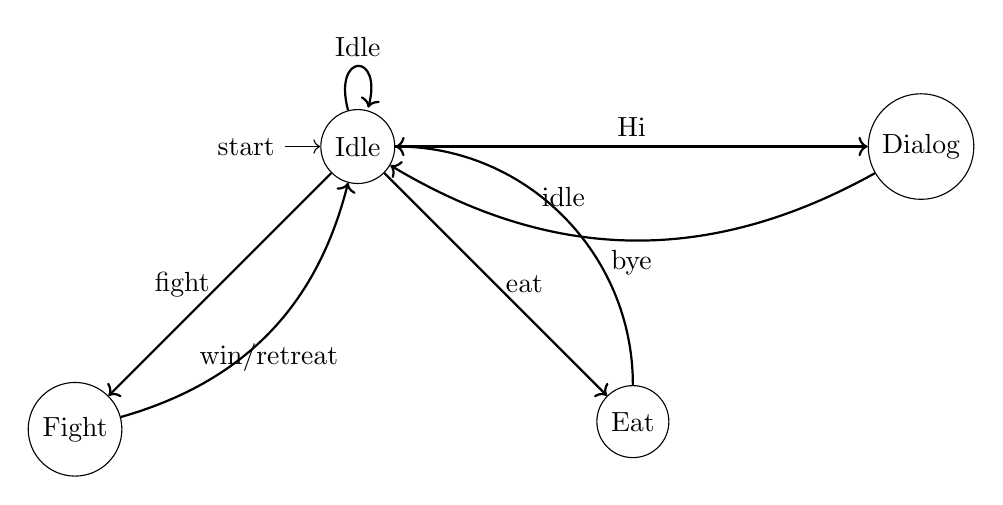
\begin{tikzpicture}[node distance=6cm]
  \node[state,initial] (Idle)   {Idle};
  \node[state]         (Dialog) [right=of Idle]            {Dialog};
  \node[state]         (Fight)  [below left=4cm of Idle]   {Fight};
  \node[state]         (Eat)    [below right=4cm of Idle]  {Eat};

  \path[->,thick]
    (Idle)   edge                node[above]{Hi}            (Dialog)
    (Idle)   edge[loop above]    node        {Idle}         ()
    (Idle)   edge                node[left] {fight}         (Fight)
    (Idle)   edge                node[right]{eat}           (Eat)
    (Dialog) edge[bend left=30]  node[below]{bye}           (Idle)
    (Eat)    edge[bend right=45] node[above]{idle}          (Idle)
    (Fight)  edge[bend right=30] node[below]{win/retreat}   (Idle);
\end{tikzpicture}
\end{center}

%--------------------------------------------------------------------
\subsection*{Impa's Simple Dialog Automaton}

\begin{center}
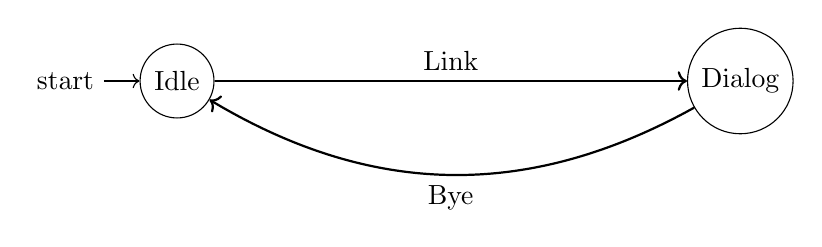
\begin{tikzpicture}[node distance=6cm]
  \node[state,initial] (IdleI)  {Idle};
  \node[state]         (DialogI)[right=of IdleI] {Dialog};

  \path[->,thick]
    (IdleI)   edge               node[above]{Link} (DialogI)
    (DialogI) edge[bend left=30] node[below]{Bye}  (IdleI);
\end{tikzpicture}
\end{center}

%--------------------------------------------------------------------
\subsection*{Zelda's Simple Dialog Automaton}

\begin{center}
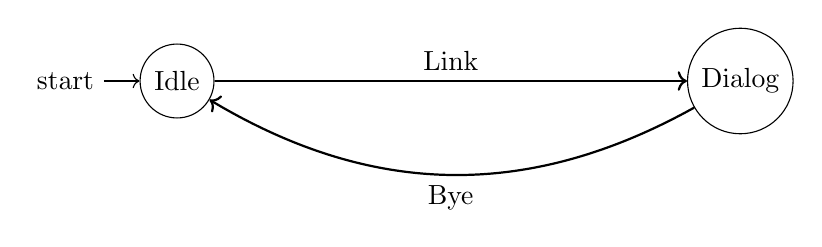
\begin{tikzpicture}[node distance=6cm]
  \node[state,initial] (IdleZ)  {Idle};
  \node[state]         (DialogZ)[right=of IdleZ] {Dialog};

  \path[->,thick]
    (IdleZ)   edge               node[above]{Link} (DialogZ)
    (DialogZ) edge[bend left=30] node[below]{Bye}  (IdleZ);
\end{tikzpicture}
\end{center}

%--------------------------------------------------------------------
\subsection*{Ganon's Battle Automaton}

\begin{center}
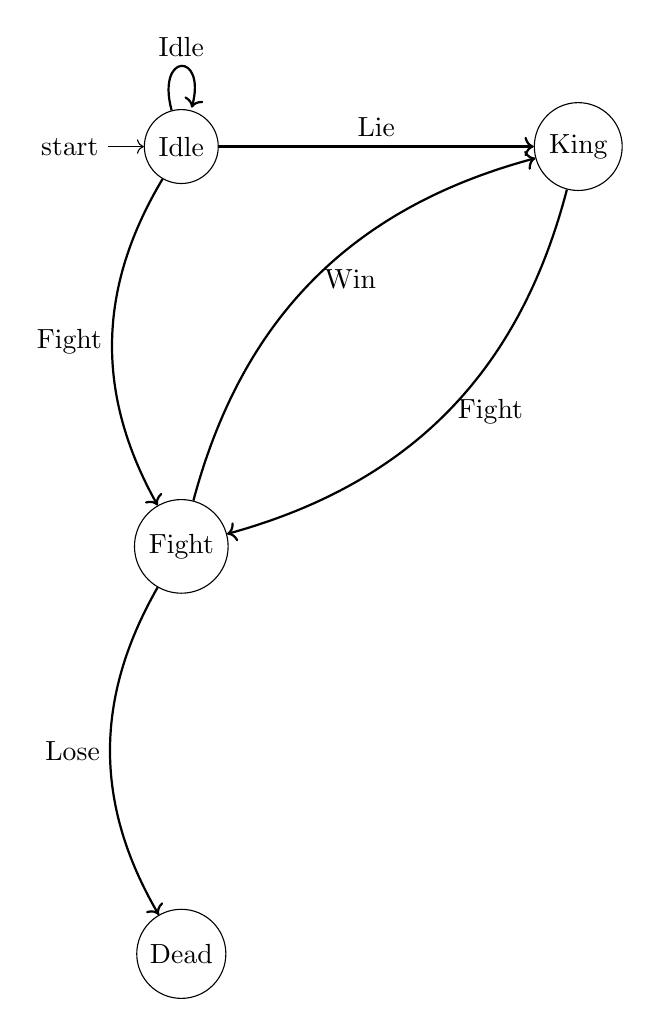
\begin{tikzpicture}[node distance=4cm]
  \node[state,initial] (IdleG)  {Idle};
  \node[state]         (King)   [right=of IdleG] {King};
  \node[state]         (FightG) [below=of IdleG] {Fight};
  \node[state]         (Dead)   [below=of FightG]{Dead};

  \path[->,thick]
    (IdleG)  edge               node[above]{Lie}   (King)
    (IdleG)  edge[loop above]   node        {Idle} ()
    (IdleG)  edge[bend right]    node[left] {Fight} (FightG)
    (King)   edge[bend left]    node[right]{Fight} (FightG)
    (FightG) edge[bend left]    node[right]{Win}   (King)
    (FightG) edge[bend right]    node[left]{Lose}  (Dead);
\end{tikzpicture}
\end{center}

%--------------------------------------------------------------------
\pagebreak
\subsection*{Impa’s NFA Dialog}

\begin{center}
\begin{figure}[ht]
    \centering % centers the figure   
    \begin{tikzpicture}[node distance=2.5cm, ->, >=stealth']
        \node[state, initial] (q0) {$q_0$};
        \node[state, right of=q0] (q1) {$q_1$};
        \node[state, right of=q1] (q2) {$q_2$};
        \node[state, right of=q2] (q3) {$q_3$};
        \node[state, below of=q2] (q4) {$q_4$};
        \node[state, below of=q3] (q5) {$q_5$};
        \node[state, right of=q5, accepting] (q6) {$q_6$};
        \draw (q0) edge[below, bend right] node{$E$} (q1)
              (q1) edge[above, bend right] node{$T$} (q0)
              (q1) edge[above] node{$Y$} (q2)
              (q1) edge[left] node{$N$} (q4)
              (q2) edge[above] node{$Q$} (q3)
              (q3) edge[right] node{$B$} (q5)
              (q4) edge[above] node{$B$} (q5)
              (q5) edge[above] node{$B$} (q6)
    \end{tikzpicture}
    \caption{NFA of accepted dialog between Link and Impa}
    \label{fig:my_label}
\end{figure}
\end{center}
%--------------------------------------------------------------------
\subsection*{Impa – language and grammar}

L = {E(TE)*(YQ|N)(BB)}

%--------------------------------------------------------------------
\pagebreak
\subsection*{Zelda’s NFA Dialog }

\begin{center}
\begin{figure}[ht]
    \centering % centers the figure   
    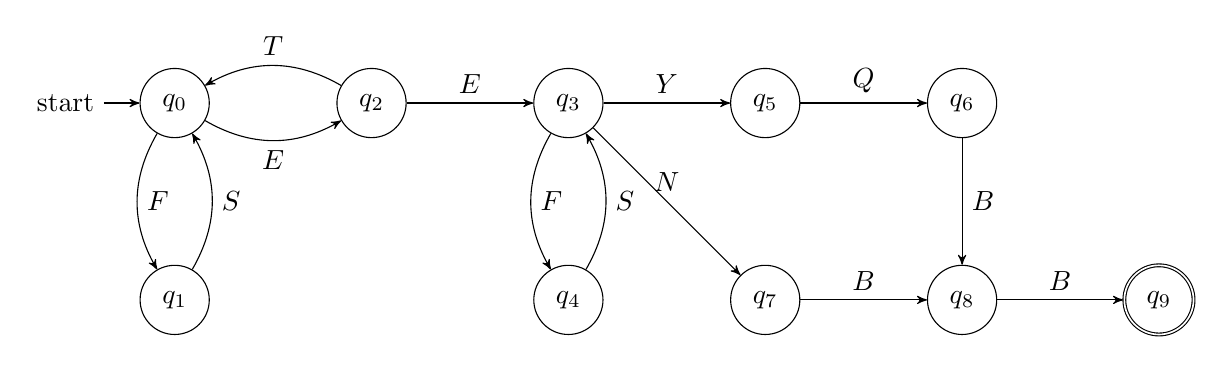
\begin{tikzpicture}[node distance=2.5cm, ->, >=stealth']
        \node[state, initial] (q0) {$q_0$};
        \node[state, below of=q0] (q1) {$q_1$};
        \node[state, right of=q0] (q2) {$q_2$};
        \node[state, right of=q2] (q3) {$q_3$};
        \node[state, below of=q3] (q4) {$q_4$};
        \node[state, right of=q3] (q5) {$q_5$};
        \node[state, right of=q5] (q6) {$q_6$};
        \node[state, right of=q4] (q7) {$q_7$};
        \node[state, right of=q7] (q8) {$q_8$};
        \node[state, right of=q8, accepting] (q9) {$q_9$};
        \draw (q0) edge[below, bend right] node{$E$} (q2)
              (q0) edge[left, bend right, right=.1] node{$F$} (q1)
              (q1) edge[right, bend right, right=.1] node{$S$} (q0)
              (q2) edge[above, bend right] node{$T$} (q0)
              (q2) edge[above] node{$E$} (q3)
              (q3) edge[left, bend right, right=.1] node{$F$} (q4)
              (q3) edge[above] node{$Y$} (q5)
              (q3) edge[above] node{$N$} (q7)
              (q4) edge[right, bend right, right=.1] node{$S$} (q3)
              (q5) edge[above] node{$Q$} (q6)
              (q6) edge[right] node{$B$} (q8)
              (q7) edge[above] node{$B$} (q8)
              (q8) edge[above] node{$B$} (q9);
    \end{tikzpicture}
    \caption{NFA of accepted dialog between Link and Zelda}
    \label{fig:my_label}
\end{figure}
\end{center}
%--------------------------------------------------------------------

\subsection*{Zelda – language and grammar}

L = {E(FS)*(TE(FS)*)*(YQ|B)(BB)}

%--------------------------------------------------------------------
\subsection*{Bokoblin State Machine}

\begin{center}
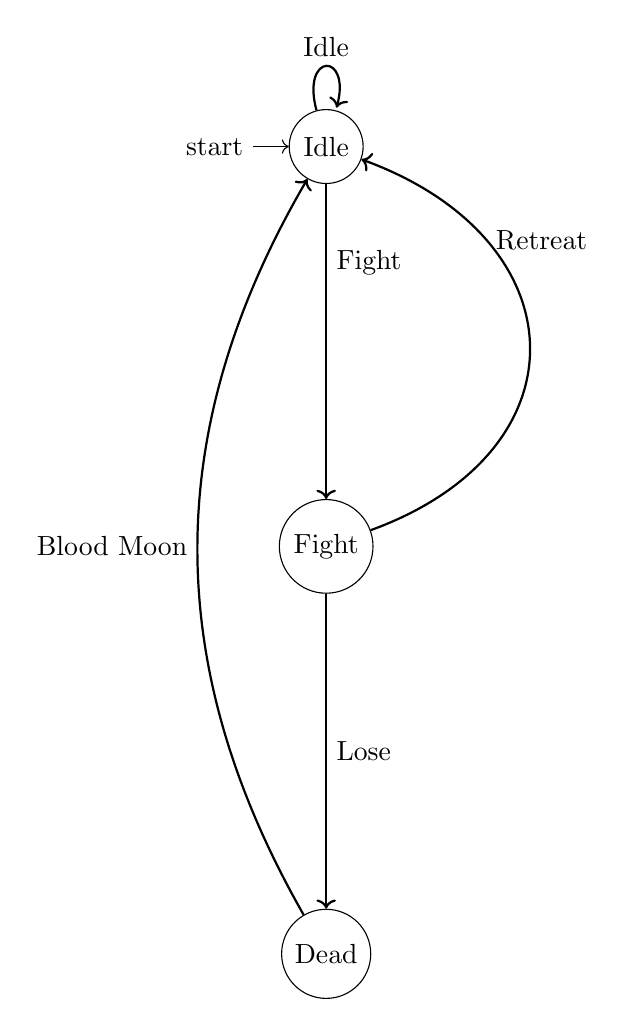
\begin{tikzpicture}[node distance=4cm]
  \node[state, initial] (IdleB)  {Idle};
  \node[state]          (FightB) [below=of IdleB] {Fight};
  \node[state]          (DeadB)  [below=of FightB]{Dead};

  \path[->,thick]
    (IdleB) edge[loop above] node{Idle} ()
    (IdleB) edge node[pos=.25, right]{Fight} (FightB)
    (FightB) edge[out=20,in=-20,looseness=1.6]
              node[pos=.75,right]{Retreat} (IdleB)
    (DeadB) edge[bend left]
              node[left]{Blood Moon} (IdleB)
    (FightB) edge              node[right]{Lose} (DeadB);
\end{tikzpicture}
\end{center}

\subsection*{Link Fighting}

\begin{center}
\scalebox{0.7}{
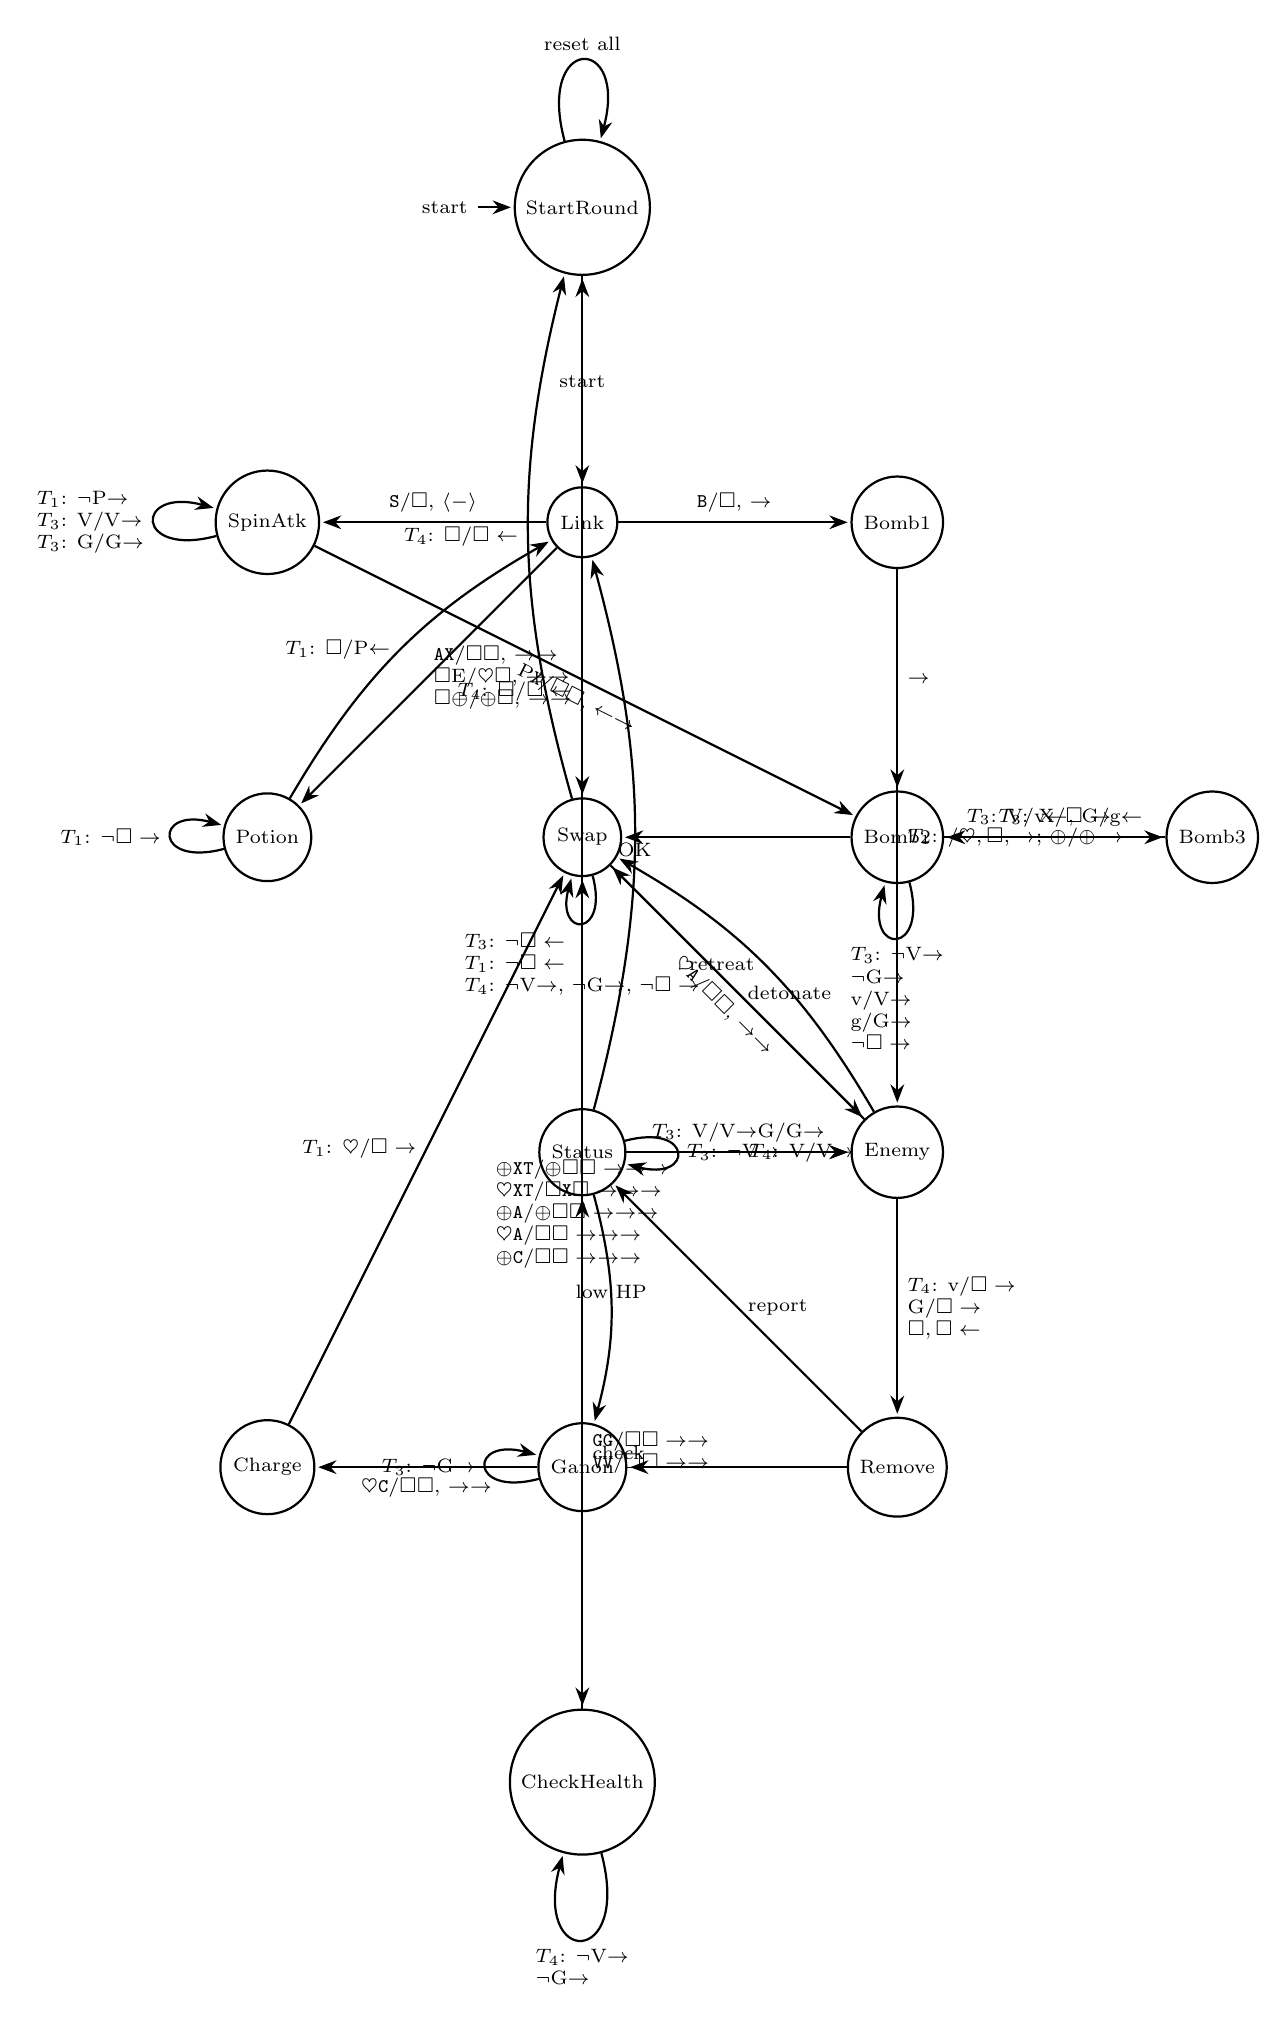
\begin{tikzpicture}[
    >=Stealth,
    ->,
    thick,
    shorten >=1pt,
    every node/.style={font=\scriptsize},
    every edge/.style={font=\tiny, pos=0.5, draw}
]

% ---------------- States ----------------
\node[state,initial] (sr) at (0,0) {Start\\Round};
\node[state] (lk) at (0,-4) {Link};
\node[state] (spin) at (-4,-4) {Spin\\Atk};
\node[state] (b1) at (4,-4) {Bomb1};
\node[state] (b2) at (4,-8) {Bomb2};
\node[state] (b3) at (8,-8) {Bomb3};
\node[state] (sw) at (0,-8) {Swap};
\node[state] (pot) at (-4,-8) {Potion};
\node[state] (enm) at (4,-12) {Enemy};
\node[state] (rm) at (4,-16) {Remove};
\node[state] (gn) at (0,-16) {Ganon};
\node[state] (chg) at (-4,-16) {Charge};
\node[state] (st) at (0,-12) {Status};
\node[state] (chk) at (0,-20) {Check\\Health};

% ---------------- Transitions ----------------
% Start Round
\draw[->] (sr) edge[loop above] node{reset all} ()
          (sr) edge node{start} (lk);

% Link
\draw[->] (lk) edge node[above,sloped]{\texttt{B}/$\square$, $\rightarrow$} (b1)
          (lk) edge node[above,sloped]{\texttt{S}/$\square$, $\langle-\rangle$} (spin)
          (lk) edge node[left,align=left]{
              \texttt{AX}/$\square\square$, $\rightarrow\rightarrow$\\
              $\square$E/$\heartsuit\square$, $\rightarrow\rightarrow$\\
              $\square\oplus$/$\oplus\square$, $\rightarrow\rightarrow$
          } (sw)
          (lk) edge node{} (pot);

% Spin Attack
\draw[->] (spin) edge[loop left] node[left,align=left]{
                  $T_1$: $\lnot$P$\rightarrow$\\
                  $T_3$: V/V$\rightarrow$\\
                  $T_3$: G/G$\rightarrow$
              } ()
             (spin) edge node[below,sloped]{P\texttt{X}/$\square\square$, $\leftarrow\rightarrow$} (b2);

% Bomb1
\draw[->] (b1) edge node[right]{$T_1$: /$\heartsuit,\square,\rightarrow$; $\oplus/\oplus\rightarrow$} (enm)
          (b1) edge node[right]{$\rightarrow$} (b2);

% Bomb2
\draw[->] (b2) edge[loop below] node[below,align=left]{
                  $T_3$: $\lnot$V$\rightarrow$\\
                  $\lnot$G$\rightarrow$\\
                  v/V$\rightarrow$\\
                  g/G$\rightarrow$\\
                  $\lnot\square\rightarrow$
              } ()
           (b2) edge node[above]{$T_3$: V/v$\leftarrow$, G/g$\leftarrow$} (b3)
           (b2) edge node{} (sw);

% Bomb3
\draw[->] (b3) edge node[above]{$T_3$: X/$\square\rightarrow$} (b2);

% Potion
\draw[->] (pot) edge[loop left] node[left]{$T_1$: $\lnot\square\rightarrow$} ()
           (pot) edge[bend left=15] node[left]{$T_1$: $\square$/P$\leftarrow$} (lk);

% Swap
\draw[->] (sw) edge node[right]{detonate} (enm)
          (sw) edge[loop below] node[below,align=left]{
                  $T_3$: $\lnot\square\leftarrow$\\
                  $T_1$: $\lnot\square\leftarrow$\\
                  $T_4$: $\lnot$V$\rightarrow$, $\lnot$G$\rightarrow$, $\lnot\square\rightarrow$
              } ()
          (sw) edge[bend left=15] node[left]{$T_4$: $\square/\square\leftarrow$} (sr);

% Enemy
\draw[->] (enm) edge[bend right=15] node[left]{retreat} (sw)
           (enm) edge node[below,sloped]{$\heartsuit$\texttt{A}/$\square\square$, $\rightarrow\rightarrow$} (sw)
           (enm) edge node[right,align=left]{
               $T_4$: v/$\square\rightarrow$\\
               G/$\square\rightarrow$\\
               $\square,\square\leftarrow$
           } (rm);

% Remove
\draw[->] (rm) edge node[right]{report} (st)
          (rm) edge (gn);

% Ganon
\draw[->] (gn) edge[loop left] node[left]{$T_3$: $\lnot$G$\rightarrow$} ()
          (gn) edge node[below,sloped]{$\heartsuit$\texttt{C}/$\square\square$, $\rightarrow\rightarrow$} (chg)
          (gn) edge node[below,align=left]{
              $\oplus$\texttt{XT}/$\oplus\square\square\rightarrow\rightarrow\rightarrow$\\
              $\heartsuit$\texttt{XT}/$\square$\texttt{X}$\square\rightarrow\rightarrow\rightarrow$\\
              $\oplus$\texttt{A}/$\oplus\square\square\rightarrow\rightarrow\rightarrow$\\
              $\heartsuit$\texttt{A}/$\square\square\rightarrow\rightarrow\rightarrow$\\
              $\oplus$\texttt{C}/$\square\square\rightarrow\rightarrow\rightarrow$
          } (sw);

% Charge
\draw[->] (chg) edge node[left]{$T_1$: $\heartsuit/\square\rightarrow$} (sw);

% Status
\draw[->] (st) edge node[right]{$T_4$: V/V$\rightarrow$} (enm)
          (st) edge node[above,sloped]{$T_3$: V/V$\rightarrow$\\G/G$\rightarrow$} (enm)
          (st) edge node[left]{$T_4$: $\square/\square\leftarrow$} (sr)
          (st) edge[loop right] node[right]{$T_3$: $\lnot$V$\rightarrow$} ()
          (st) edge[bend left=15] node[above]{low HP} (gn)
          (st) edge[bend right=15] node[below]{OK} (lk)
          (st) edge node[right]{check} (chk);

% Check Health
\draw[->] (chk) edge[loop below] node[below,align=left]{
                  $T_4$: $\lnot$V$\rightarrow$\\
                  $\lnot$G$\rightarrow$
              } ()
           (chk) edge node[right,align=left]{
               \texttt{GG}/$\square\square\rightarrow\rightarrow$\\
               \texttt{VV}/$\square\square\rightarrow\rightarrow$
           } (st);

\end{tikzpicture}
}
\end{center}
\end{document}